\section{Lady of Shalott}

\label{sec:LadyShallot}

\begin{quotex}
To all the knights of the Round Table sends health this lady of Shalott, as to the best people of the world. And if you want to know why I came to my end, that is because of the greatest knight in the world, and the most ungracious; that is my lord Sir Lancelot of the Lake, whom I was unable to pray of his love such that he would have pity of me. And thus, weary, I died, for loving well, as you can see!
\flright{\textit{Final letter of the Lady of Shalott}}

\end{quotex}
In the \textbf{Matter of Britain}, the \textbf{Lady of Shalott} was \textbf{Elaine of Astolat}. Elaine was in love with Lancelot. When the knight was injured in battle, she nursed him back to health. After he recovered, he treated her like hired help, unaware of her feelings for him. Her love unrequited, she died of heartbreak ten days later.

\begin{wrapfigure}{rt}{.43\textwidth}
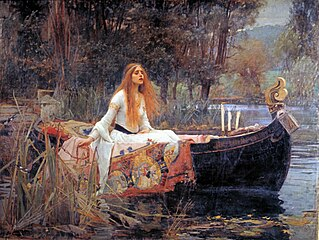
\includegraphics[scale=.45]{a20211214LadyofShalott-img001.jpg}
\end{wrapfigure} 

At that time, people participated in the world by experience unironically, not as they do today. Thus, they ``felt" the world, with emotions that were more deeply and strongly experienced, with a range that exceeds the limited emotional responses of our time.

So the story is plausible to me, since I witnessed my mother die about 10 days after my father with the same disease: heartache. At least they had a lifetime together. Lancelot spurned such a strong love that was freely offered to him. Elaine had no more reason to live.

Alfred, Lord Tennyson retold the story in the poem \textit{The Lady of Shalott}, of which he published two versions.

\hfill

\setcolumnwidth{0.55\textwidth,0.55\textwidth}
\begin{paracol}{2}\footnotesize
\settowidth{\versewidth}{The sunbeam showers break and quiver,,}
\begin{verse}[\versewidth]
\textbf{Part I} (1832)
\indentpattern{0000010001}
\begin{patverse}
\phantom{.}\\
On either side the river lie\\
Long fields of barley and of rye,\\
That clothe the wold and meet the sky;\\
And thro' the field the road runs by\\
To many-tower'd Camelot;\\
The yellow-leaved waterlily\\
The green-sheathed daffodilly\\
Tremble in the water chilly\\
Round about Shalott.
\end{patverse}

\indentpattern{000010001}\begin{patverse}
Willows whiten, aspens shiver.\\
The sunbeam showers break and quiver\\
In the stream that runneth ever\\
By the island in the river\\
Flowing down to Camelot.\\
Four gray walls, and four gray towers\\
Overlook a space of flowers,\\
And the silent isle imbowers\\
The Lady of Shalott.
\end{patverse}

\begin{patverse}
Underneath the bearded barley,\\
The reaper, reaping late and early,\\
Hears her ever chanting cheerly,\\
Like an angel, singing clearly,\\
O'er the stream of Camelot.\\
Piling the sheaves in furrows airy,\\
Beneath the moon, the reaper weary\\
Listening whispers, ``Tis the fairy,\\
Lady of Shalott.''
\end{patverse}

\begin{patverse}
The little isle is all inrail'd\\
With a rose-fence, and overtrail'd\\
With roses: by the marge unhail'd\\
The shallop flitteth silken sail'd,\\
Skimming down to Camelot.\\
A pearl garland winds her head:\\
She leaneth on a velvet bed,\\
Full royally apparelled,\\
The Lady of Shalott.\end{patverse}  \switchcolumn

\textbf{Part I} (1842)\\
\begin{patverse}
On either side the river lie\\
Long fields of barley and of rye,\\
That clothe the wold and meet the sky;\\
And thro' the field the road runs by\\
To many-tower'd Camelot;\\
And up and down the people go,\\
Gazing where the lilies blow\\
Round an island there below,\\
The island of Shalott.
\end{patverse}

\begin{patverse}
Willows whiten, aspens quiver,\\
Little breezes dusk and shiver\\
Thro' the wave that runs for ever\\
By the island in the river\\
Flowing down to Camelot.\\
Four gray walls, and four gray towers,\\
Overlook a space of flowers,\\
And the silent isle imbowers\\
The Lady of Shalott.
\end{patverse}

\begin{patverse}
By the margin, willow veil'd,\\
Slide the heavy barges trail'd\\
By slow horses; and unhail'd\\
The shallop flitteth silken-sail'd\\
Skimming down to Camelot:\\
But who hath seen her wave her hand?\\
Or at the casement seen her stand?\\
Or is she known in all the land,\\
The Lady of Shalott?
\end{patverse}

\begin{patverse}
Only reapers, reaping early\\
In among the bearded barley,\\
Hear a song that echoes cheerly\\
From the river winding clearly,\\
Down to tower'd Camelot:\\
And by the moon the reaper weary,\\
Piling sheaves in uplands airy,\\
Listening, whispers ``Tis the fairy\\
Lady of Shalott." \end{patverse}\switchcolumn

\textbf{Part II}
\indentpattern{0000010001}\begin{patverse}
\phantom{.}\\
No time hath she to sport and play:\\
A charmed web she weaves alway.\\
A curse is on her, if she stay\\
Her weaving, either night or day,\\
To look down to Camelot.\\
She knows not what the curse may be;\\
Therefore she weaveth steadily,\\
Therefore no other care hath she,\\
The Lady of Shalott.
\end{patverse}

\indentpattern{000010001}\begin{patverse}
She lives with little joy or fear.\\
Over the water, running near,\\
The sheepbell tinkles in her ear.\\
Before her hangs a mirror clear,\\
Reflecting tower'd Camelot.\\
And as the mazy web she whirls,\\
She sees the surly village churls,\\
And the red cloaks of market girls\\
Pass onward from Shalott.
\end{patverse}

\begin{patverse}
Sometimes a troop of damsels glad,\\
An abbot on an ambling pad,\\
Sometimes a curly shepherd lad,\\
Or long-hair'd page in crimson clad,\\
Goes by to tower'd Camelot:\\
And sometimes thro' the mirror blue\\
The knights come riding two and two:\\
She hath no loyal knight and true,\\
The Lady of Shalott.
\end{patverse}

\begin{patverse}
But in her web she still delights\\
To weave the mirror's magic sights,\\
For often thro' the silent nights\\
A funeral, with plumes and lights\\
And music, came from Camelot:\\
Or when the moon was overhead\\
Came two young lovers lately wed;\\
`I am half sick of shadows,' said\\
The Lady of Shalott.  \end{patverse}\switchcolumn

\textbf{Part II}
\indentpattern{0000010001}\begin{patverse}
\phantom{.}\\
There she weaves by night and day\\
A magic web with colours gay.\\
She has heard a whisper say,\\
A curse is on her if she stay\\
To look down to Camelot.\\
She knows not what the curse may be,\\
And so she weaveth steadily,\\
And little other care hath she,\\
The Lady of Shalott.
\end{patverse}

\indentpattern{000010001}\begin{patverse}
And moving thro' a mirror clear\\
That hangs before her all the year,\\
Shadows of the world appear.\\
There she sees the highway near\\
Winding down to Camelot:\\
There the river eddy whirls,\\
And there the surly village-churls,\\
And the red cloaks of market girls,\\
Pass onward from Shalott.
\end{patverse}

\begin{patverse}
Sometimes a troop of damsels glad,\\
An abbot on an ambling pad,\\
Sometimes a curly shepherd-lad,\\
Or long-hair'd page in crimson clad,\\
Goes by to tower'd Camelot;\\
And sometimes thro' the mirror blue\\
The knights come riding two and two:\\
She hath no loyal knight and true,\\
The Lady of Shalott.
\end{patverse}

\begin{patverse}
But in her web she still delights\\
To weave the mirror's magic sights,\\
For often thro' the silent nights\\
A funeral, with plumes and lights\\
And music, went to Camelot:\\
Or when the moon was overhead,\\
Came two young lovers lately wed:\\
``I am half sick of shadows," said\\
The Lady of Shalott. \end{patverse}\switchcolumn

\textbf{Part III}
\indentpattern{0000010001}\begin{patverse}
\phantom{.}\\
A bow-shot from her bower-eaves,\\
He rode between the barley-sheaves,\\
The sun came dazzling thro' the leaves,\\
And flam'd upon the brazen greaves\\
Of bold Sir Lancelot.\\
A red-cross knight for ever kneel'd\\
To a lady in his shield,\\
That sparkled on the yellow field,\\
Beside remote Shalott.
\end{patverse}

\indentpattern{000010001}\begin{patverse}
The gemmy bridle glitter'd free,\\
Like to some branch of stars we see\\
Hung in the golden Galaxy.\\
The bridle bells rang merrily\\
As he rode down from Camelot:\\
And from his blazon'd baldric slung\\
A mighty silver bugle hung,\\
And as he rode his armour rung,\\
Beside remote Shalott.
\end{patverse}

\begin{patverse}
All in the blue unclouded weather\\
Thick-jewell'd shone the saddle-leather,\\
The helmet and the helmet-feather\\
Burn'd like one burning flame together,\\
As he rode down from Camelot.\\
As often thro' the purple night,\\
Below the starry clusters bright,\\
Some bearded meteor, trailing light,\\
Moves over green Shalott.
\end{patverse}

\begin{patverse}
His broad clear brow in sunlight glow'd;\\
On burnish'd hooves his war-horse trode;\\
From underneath his helmet flow'd\\
His coal-black curls as on he rode,\\
As he rode down from Camelot.\\
From the bank and from the river\\
He flash'd into the crystal mirror,\\
`Tirra lirra, tirra lirra:'\\
Sang Sir Lancelot.
\end{patverse}

\begin{patverse}
She left the web, she left the loom\\
She made three paces thro' the room\\
She saw the water-flower bloom,\\
She saw the helmet and the plume,\\
She look'd down to Camelot.\\
Out flew the web and floated wide;\\
The mirror crack'd from side to side;\\
`The curse is come upon me,' cried\\
The Lady of Shalott.\end{patverse}  \switchcolumn

\textbf{Part III}
\indentpattern{0000010001}\begin{patverse}
\phantom{.}\\
A bow-shot from her bower-eaves,\\
He rode between the barley-sheaves,\\
The sun came dazzling thro' the leaves,\\
And flamed upon the brazen greaves\\
Of bold Sir Lancelot.\\
A red-cross knight for ever kneel'd\\
To a lady in his shield,\\
That sparkled on the yellow field,\\
Beside remote Shalott.
\end{patverse}

\indentpattern{000010001}\begin{patverse}
The gemmy bridle glitter'd free,\\
Like to some branch of stars we see\\
Hung in the golden Galaxy.\\
The bridle bells rang merrily\\
As he rode down to Camelot:\\
And from his blazon'd baldric slung\\
A mighty silver bugle hung,\\
And as he rode his armour rung,\\
Beside remote Shalott.
\end{patverse}

\begin{patverse}
All in the blue unclouded weather\\
Thick-jewell'd shone the saddle-leather,\\
The helmet and the helmet-feather\\
Burn'd like one burning flame together,\\
As he rode down to Camelot.\\
As often thro' the purple night,\\
Below the starry clusters bright,\\
Some bearded meteor, trailing light,\\
Moves over still Shalott.
\end{patverse}

\begin{patverse}
His broad clear brow in sunlight glow'd;\\
On burnish'd hooves his war-horse trode;\\
From underneath his helmet flow'd\\
His coal-black curls as on he rode,\\
As he rode down to Camelot.\\
From the bank and from the river\\
He flash'd into the crystal mirror,\\
``Tirra lirra," by the river\\
Sang Sir Lancelot.
\end{patverse}

\begin{patverse}
She left the web, she left the loom,\\
She made three paces thro' the room,\\
She saw the water-lily bloom,\\
She saw the helmet and the plume,\\
She look'd down to Camelot.\\
Out flew the web and floated wide;\\
The mirror crack'd from side to side;\\
``The curse is come upon me," cried\\
The Lady of Shalott.\end{patverse} \switchcolumn

\textbf{Part IV}
\indentpattern{0000010001}\begin{patverse}
\phantom{.}\\
In the stormy east-wind straining,\\
The pale yellow woods were waning,\\
The broad stream in his banks complaining,\\
Heavily the low sky raining\\
Over tower'd Camelot;\\
Outside the isle a shallow boat\\
Beneath a willow lay afloat,\\
Below the carven stern she wrote,\\
\emph{The Lady of Shalott.}
\end{patverse}

\begin{patverse}
A cloudwhite crown of pearl she dight,\\
All raimented in snowy white\\
That loosely flew (her zone in sight\\
Clasp'd with one blinding diamond bright\\
Her wide eyes fix'd on Camelot,\\
Though the squally east-wind keenly\\
Blew, with folded arms serenely\\
By the water stood the queenly\\
Lady of Shalott.
\end{patverse}

\begin{patverse}
With a steady stony glance—\\
Like some bold seer in a trance,\\
Beholding all his own mischance,\\
Mute, with a glassy countenance—\\
She look'd down to Camelot.\\
It was the closing of the day:\\
She loos'd the chain, and down she lay;\\
The broad stream bore her far away,\\
The Lady of Shalott.
\end{patverse}

\begin{patverse}
As when to sailors while they roam,\\
By creeks and outfalls far from home,\\
Rising and dropping with the foam,\\
From dying swans wild warblings come,\\
Blown shoreward; so to Camelot\\
Still as the boathead wound along\\
The willowy hills and fields among,\\
They heard her chanting her deathsong,\\
The Lady of Shalott.
\end{patverse}

\begin{patverse}
A longdrawn carol, mournful, holy,\\
She chanted loudly, chanted lowly,\\
Till her eyes were darken'd wholly,\\
And her smooth face sharpen'd slowly,\\
Turn'd to tower'd Camelot:\\
For ere she reach'd upon the tide\\
The first house by the water-side,\\
Singing in her song she died,\\
The Lady of Shalott.
\end{patverse}

\begin{patverse}
Under tower and balcony,\\
By garden wall and gallery,\\
A pale, pale corpse she floated by,\\
Deadcold, between the houses high,\\
Dead into tower'd Camelot.\\
Knight and burgher, lord and dame,\\
To the planked wharfage came:\\
Below the stern they read her name,\\
\emph{The Lady of Shalott.}
\end{patverse}

\begin{patverse}
They cross'd themselves, their stars they blest,\\
Knight, minstrel, abbot, squire, and guest.\\
There lay a parchment on her breast,\\
That puzzled more than all the rest,\\
The wellfed wits at Camelot.\\
`The web was woven curiously,\\
The charm is broken utterly,\\
Draw near and fear not, —this is I,\\
The Lady of Shalott.' \end{patverse} \switchcolumn

\textbf{Part IV} 
\indentpattern{0000010001}\begin{patverse}
\phantom{.}\\
In the stormy east-wind straining,\\
The pale yellow woods were waning,\\
The broad stream in his banks complaining,\\
Heavily the low sky raining\\
Over tower'd Camelot;\\
Down she came and found a boat\\
Beneath a willow left afloat,\\
And round about the prow she wrote\\
\emph{The Lady of Shalott.}
\end{patverse}

\indentpattern{000010001}\begin{patverse}
And down the river's dim expanse\\
Like some bold seër in a trance,\\
Seeing all his own mischance—\\
With a glassy countenance\\
Did she look to Camelot.\\
And at the closing of the day\\
She loosed the chain, and down she lay;\\
The broad stream bore her far away,\\
The Lady of Shalott.
\end{patverse}

\begin{patverse}
Lying, robed in snowy white\\
That loosely flew to left and right—\\
The leaves upon her falling light—\\
Thro' the noises of the night\\
She floated down to Camelot:\\
And as the boat-head wound along\\
The willowy hills and fields among,\\
They heard her singing her last song,\\
The Lady of Shalott.
\end{patverse}

\begin{patverse}
Heard a carol, mournful, holy,\\
Chanted loudly, chanted lowly,\\
Till her blood was frozen slowly,\\
And her eyes were darken'd wholly,\\
Turn'd to tower'd Camelot.\\
For ere she reach'd upon the tide\\
The first house by the water-side,\\
Singing in her song she died,\\
The Lady of Shalott.
\end{patverse}

\begin{patverse}
Under tower and balcony,\\
By garden-wall and gallery,\\
A gleaming shape she floated by,\\
Dead-pale between the houses high,\\
Silent into Camelot.\\
Out upon the wharfs they came,\\
Knight and burgher, lord and dame,\\
And round the prow they read her name,\\
\emph{The Lady of Shalott.}
\end{patverse}

\begin{patverse}
Who is this? and what is here?\\
And in the lighted palace near\\
Died the sound of royal cheer;\\
And they cross'd themselves for fear,\\
All the knights at Camelot:\\
But Lancelot mused a little space;\\
He said, ``She has a lovely face;\\
God in his mercy lend her grace,\\
The Lady of Shalott."
\end{patverse}
\end{verse}
\end{paracol}
\paragraph{Appendix: An Anima Dream}
Last night, I had another Anima dream, which surprised me. I spotted a woman at a gathering. I recognized her from some other time, maybe even from a different turn of the spiral of the degrees of Existence. As I sat in an armchair, she approached and sat on my lap. Then she gently kissed me on my lips. There was such joy, like the ending of Sehnsucht, that I felt it even in my sleep. I vowed never to pass up such love again.

\url{https://www.youtube.com/watch?v=DRIHzr3Pxhc}



\flrightit{Posted on 2021-12-14 by Cologero }
